\chapter{Распространение ключей}\index{протокол!распространения ключей}
\selectlanguage{russian}

Задачей распространения ключей между двумя пользователями является создание секретных псевдослучайных сеансовых ключей шифрования и аутентификация сообщений. Пользователи предварительно создают и обмениваются ключами аутентификации один раз. В дальнейшем для создания защищенной связи пользователи производят взаимную аутентификацию и вырабатывают сеансовые ключи\index{ключ!сеансовый}.

\section[Трёхэтапный протокол Шамира]{Трёхэтапный протокол Шамира на коммутативных шифрах}
\selectlanguage{russian}

Предположим, что две стороны $A$ и $B$ соединены незащищённым каналом связи. Каждая из этих сторон имеет свой секретный ключ: $A$ имеет ключ $K_A$, $B$ имеет ключ $K_B$. Сторона $A$ должна создать общий секретный ключ $K$ и передать стороне $B$.

Для решения этой задачи используют трёхэтапный протокол Шамира с тремя <<замками>>. \textbf{Протокол Шамира}\index{протокол!Шамира} построен на \emph{коммутативных} функциях шифрования, для которых выполняется условие:
    \[ E_{K_{B}} (E_{K_{A}}(K))=E_{K_{A}} (E_{K_{B}}(K)). \]

Протокол предполагает следующие процедуры.
\begin{enumerate}
    \item $A$ создаёт секретный ключ $K$, шифрует его своей системой шифрования с помощью своего ключа $K_A$ и посылает сообщение стороне $B$:
        \[ A \rightarrow B: ~ E_{K_A}(K). \]
    \item $B$ получает это сообщение, шифрует его с помощью своего ключа $K_B$ и посылает сообщение стороне $A$:
        \[ A \leftarrow B: ~ E_{K_B}( E_{K_A}( K)). \]
    \item Сторона $A$, получив сообщение $E_{K_B}(E_{K_A}(K))$, использует свой секретный ключ $K_A$ для расшифрования:
            \[ D_{K_A}(E_{K_B} (E_{K_A}(K))) = E_{K_B}(K). \]
        Сторона $A$ передаёт стороне $B$ сообщение:
        \[ A \rightarrow B: ~ E_{K_B}(K). \]
    \item Сторона $B$, получив сообщение $E_{K_B}(K)$, использует свой секретный ключ $K_B$ для расшифрования:
            \[ D_{K_B}(E_{K_B}(K)) = K. \]
        В результате стороны получают общий секретный ключ $K$.
\end{enumerate}

Приведём пример неудачного шифрования с использованием коммутативных функций.

\begin{enumerate}
    \item $A$ имеет функцию шифрования совершенной секретности $E_{K_A}(K) = K \oplus K_A$, где $K_A$ -- двоичная последовательность с равномерным распределением символов. $A$ посылает это сообщение стороне $B$:
            \[ A \rightarrow B: ~ E_{K_A}(K) = K \oplus K_A. \]
    \item $B$ использует такую же функцию шифрования совершенной секретности с ключом $K_B$ (двоичная последовательность с равномерным распределением символов). $B$ шифрует полученное сообщение и отправляет $A$:
            \[ A \leftarrow B: ~ E_{K_A}(K) \oplus K_B = K \oplus K_A \oplus K_B. \]
    \item Сторона $A$, получив сообщение $K \oplus K_A \oplus K_B$, выполняет расшифрование:
            \[ K \oplus K_A \oplus K_B \oplus K_A = K \oplus K_B. \]
        Сторона $A$ передаёт стороне $B$ сообщение:
            \[ A \rightarrow B: ~ K \oplus K_B. \]
    \item Сторона $B$, получив сообщение $K \oplus K_B$, выполняет расшифрование:
            \[ K \oplus K_B \oplus K_B = K. \]
        Обе стороны получают общий секретный ключ $K$.
\end{enumerate}

Предложенный выбор коммутативной функции шифрования совершенной секретности был назван неудачным, так как существуют ситуации, при которых криптоаналитик может определить ключ $K$. Предположим, что криптоаналитик перехватил все три сообщения:
    \[ K \oplus K_A, ~~ K \oplus K_A \oplus K_B, ~~ K \oplus K_B. \]
Сложение по модулю 2 всех трёх сообщений даёт ключ $K$. Поэтому такая система шифрования не применяется.

Теперь приведём протокол надёжной передачи секретного ключа, основанный на экспоненциальной (коммутативной) функции шифрования. Стойкость этого протокола связана с трудной задачей -- задачей вычисления дискретного логарифма: известны значения $y, g, p$, найти $x$ в уравнении $y = g^x \mod p$.

\textbf{Протокол Шамира распространения ключей.}
Выбирают большое простое\index{число!простое} число $p\sim 2^{1024}$ и используют его как открытый ключ.

\begin{enumerate}
    \item Сторона $A$ задаёт общий секретный ключ $K <p$ и выбирает целое число $a$, взаимно простое с $p-1$. $A$ вычисляет и посылает сообщение стороне $B$:
            \[ A \rightarrow B: ~ K^a \mod p. \]
        Существует число $c$ такое, что $a c =1 \mod (p-1)$, то есть $a c = 1 + l (p-1)$, где $l$ -- целое число. Число $c$ будет использовано стороной $A$ на следующем этапе.
    \item Сторона $B$ выбирает целое число $b$, взаимно простое с $p-1$. Используя полученное сообщение, вычисляет и посылает сообщение стороне $A$:
            \[ A \leftarrow B: ~ (K^a)^b \mod p. \]
    \item Сторона $A$, получив сообщение, вычисляет
        \[ \left( K^{ab} \right)^c = K^{1 + l (p-1) b} = K^b \cdot K^{l (p-1) b} = K^b \mod p. \]
        Здесь применена малая теорема Ферма\index{теорема!Ферма малая}: $K^{p-1} = 1 \mod p$, поэтому $\left( K^{p-1} \right)^{lb} = 1 \mod p$.
        $A$ посылает $B$ сообщение:
            \[ A \rightarrow B: ~ K^b \mod p. \]
    \item Сторона $B$, получив сообщение $K^{b}\mod p$, вычисляет
        \[ (K^b \mod p)^d = K^{bd} \mod p = K. \]
\end{enumerate}

Теперь проверим криптостойкость этого протокола. Предположим, что криптоаналитик перехватил три сообщения:
\[ \begin{array}{l}
    y_1 = K^a \mod p, \\
    y_2 = K^{ab} \mod p, \\
    y_3 = K^b \mod p. \\
\end{array} \]
Чтобы найти ключ $K$, надо решить систему из этих трёх уравнений, что имеет очень большую вычислительную сложность, неприемлемую с практической точки зрения, если все три числа $a, b, ab$ достаточно велики. Предположим, что $a$ (или $b$) мало. Тогда, вычисляя последовательные степени $y_3$ (или $y_1$), можно найти  $a$ (или $b$), сравнивая результат с $y_2$. Зная $a$, легко найти $a^{-1}\mod(p-1)$ и $K=(y_1)^{a^{-1}}\mod p$.

Недостатком этого протокола является отсутствие аутентификации сторон. Следовательно, нужно дополнительно использовать цифровую подпись при передаче сообщения.


\section{Симметричные протоколы}

\subsection{Аутентификация и атаки воспроизведения}

Рассмотрим такую ситуацию: обе стороны $A$ и $B$ имеют общий долговременный ключ $K_{AB}$ и симметричную систему шифрования. Нужно выработать сеансовый секретный ключ $K$. Сторона $A$ создает ключ $K$ и желает его передать стороне $B$.

\begin{enumerate}
    \item Для этого сторона $A$ с помощью общего ключа $K_{AB}$ создает и передает $B$ шифрованное сообщение:
            \[ A \rightarrow B: ~ E_{K_{AB}}(K, B, A). \]
        В этом сообщении имеются так называемые поля -- $(B,A)$ -- информация для дополнительного подтверждения.
    \item Сторона $B$, используя общий ключ $K_{AB}$, расшифровывает полученное сообщение:
            \[ D_{K_{AB}}( E_{K_{AB}}( K, B, A)) = (K, B, A). \]
        В результате сторона $B$ получает сеансовый ключ $K$ и дополнительные данные $(B,A)$.
\end{enumerate}

Недостаток этого протокола состоит в том, что криптоаналитик может перехватывать сообщения и через некоторое время переслать их стороне $A$.

Рассмотрим другие варианты решения задачи о передаче сеансового ключа.
Задача остается прежней: обе стороны $A$ и $B$ имеют общий долговременный секретный ключ $K_{AB}$, сторона $A$ должна выработать сеансовый секретный ключ $K$ и доставить стороне $B$.

Протокол включает \textbf{метки времени} -- информацию о моменте $t_A$ отправки сообщения и моменте получения сообщения $t_B$.

\begin{enumerate}
    \item Сторона $A$ вырабатывает $K$ и с помощью долговременного ключа $K_{AB}$ создает шифрованное сообщение с меткой времени $t_A$ и передает его стороне $B$:
            \[ A \rightarrow B: ~ E_{K_{AB}}(K, t_A). \]
    \item Сторона $B$ получает сообщение и расшифровывает его с помощью общего ключа:
            \[ D_{K_{AB}}( E_{K_{AB}}( K, t_A)) = (K, t_A). \]
        В результате $B$ получает $(K, t_A)$, то есть секретный ключ и метку времени. $B$ измеряет время прихода $t_B$ и интервал запаздывания. Если $|t_B - t_A| \le \delta$, то $B$ аутентифицирует $A$.
\end{enumerate}
Метка времени является одноразовой меткой и защищает от атак воспроизведения ранее записанных сообщений.

Рассмотрим другой способ передачи ключа с дополнительной информацией в виде \textbf{одноразовых случайных меток} (nonce -- number used once) вместо меток времени. Протокол передачи состоит в следующем.

\begin{enumerate}
    \item Сторона $A$ вырабатывает случайное число $r_A$, шифрует сообщение, в котором  $(r_A, A)$ -- реквизиты $A$, и передает его стороне $B$:
            \[ A \rightarrow B: ~ E_{K_{AB}}(r_A, A). \]
    \item Сторона $B$ вырабатывает сеансовый ключ $K$, создает шифрованное сообщение и посылает его $A$:
            \[ A \leftarrow B: ~ E_{K_{AB}}(K, r_A, A). \]
    \item Сторона $A$ расшифровывает полученное сообщение:
            \[ D_{K_{AB}}( E_{K_{AB}}( K, r_A, A)) = (K, r_A, A). \]
        В результате $A$ получает сеансовый ключ и подтверждение своих реквизитов, что является дополнительной аутентификацией.
\end{enumerate}

Предположим, что сторона $B$ тоже желает убедиться, что имеет дело со стороной $A$. Тогда этот протокол следует дополнить передачей реквизитов $B$. По-прежнему считаем, что у $A$ и $B$ -- общая система шифрования с долговременным секретным ключом $K_{AB}$.

\begin{enumerate}
    \item Сторона $A$ вырабатывает случайное число $r_A$, шифрует и передает стороне $B$ сообщение, в котором  $(r_A, A)$ -- реквизиты $A$:
            \[ A \rightarrow B: ~ E_{K_{AB}}(r_A, A). \]
    \item Сторона $B$ вырабатывает случайное число $r_B$ и отправляет стороне $A$ зашифрованное сообщение:
            \[ A \leftarrow B: ~ E_{K_{AB}}(K_B, r_B, r_A, A), \]
        где $K_B$ -- ключ $B$.
     \item Сторона $A$ осуществляет расшифрование
            \[ D_{K_{AB}}(E_{K_{AB}}(K_B, r_B, r_A, A)) = (K_B, r_B, r_A, A) \]
        и получает ключ $K_B$ и реквизиты $r_B, r_A, A$. Для аутентификации себя сторона $A$ создает свой ключ $K_A$ и отправляет стороне $B$ шифрованное сообщение
            \[ A \rightarrow B: ~ E_{K_{AB}}(K_A, r_B, r_A, B). \]
     \item Сторона $B$ осуществляет расшифрование
            \[ D_{K_{AB}}(E_{K_{AB}}(K_A, r_B, r_A, B)) = (K_A, r_B, r_A, B), \]
        которое определяет ключ $K_A$ и аутентифицирует $A$.
\end{enumerate}

Таким образом, обе стороны имеют в своем распоряжении ключи $K_A, K_B$ в качестве сеансовых секретных ключей.

\subsection{Протокол с ключевым кодом аутентификации}

При использовании хэш-функции $K = h(K_{A} \| K_{B})$ происходит усиление секретности. Здесь $(K_{A} \| K_{B})$ -- конкатенация $K_{A} $ и $K_{B}$.

% Достоинства: предположим, $K_{A} ,K_{B} $ -- не обладают «хорошими» свойствами случайности (биты распределены неравномерно или зависимы друг от друга), т.~е., $P_{K_{A} ,K_{B} } (0)=\frac{1}{2} -\varepsilon $, где $\varepsilon $ - мало, но не 0. Тогда вероятность того, что этот бит в \textit{K }будет равным нулю, $P_{K} (0)=\frac{1}{2} -\varepsilon ',\varepsilon '<\varepsilon $- усиление секретности.

Вычисление хэш-значения, как правило, выполняется быстрее, чем расшифрование. Поэтому были разработаны протоколы, в которых вместо функции шифрования используется имитовставка\index{имитовставка} на основе хэш-функции ($\MAC_K$). Рассмотрим протокол такого рода.
\begin{enumerate}
    \item Сторона $A$ вырабатывает сеансовый ключ $K$, использует одноразовую метку $t_{A}$, создает и пересылает стороне $B$ сообщение:
            \[ A \rightarrow B: ~ t_A, ~ B, ~ K \oplus \MAC_{K_{AB}}( t_A, B), ~ \MAC_{K_{AB}}(K, t_A, B). \]
    \item Сторона $B$ вычисляет
            \[ \MAC_{K_{AB}}(t_A, B) \oplus K \oplus \MAC_{K_{AB}}(t_A, B) = K \]
        и получает сеансовый ключ $K$.
\end{enumerate}

Заметим, что криптоаналитик может добавить в поле случайную последовательность, тогда вместо $K$ получаем <<$K$ плюс помеха>>. Вмешательство криптоаналитика будет выявлено благодаря наличию четвертого поля в сообщении. Используя полученное значение $K$, вычисляют $\MAC_{K_{AB}}(K, t_A, B)$ и сравнивают с четвертым полем. Если совпадает, то вмешательства криптоаналитика не было.

\subsection{Протокол Нидхема~---~Шрёдера}\index{протокол!Нидхема~---~Шрёдера|(}
\selectlanguage{russian}

Протокол Нидхема~---~Шрёдера (\langen{Roger Needham, Michael Shroeder}, 1979,~\cite{Needham:Schroeder:1978}) похож на модифицированный протокол Wide-Mouth Frog, но отличается тем, что доверенный центр (Трент) во время работы основной части протокола не общается со вторым абонентом. Первый абонент получает от доверенного центра специальный пакет, который он без всякой модификации отправляет второму абоненту.

\begin{figure}[!htb]
    \centering
    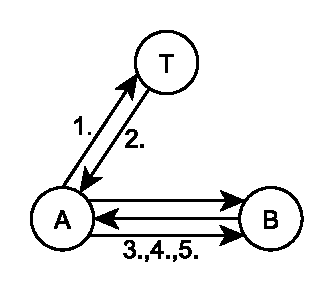
\includegraphics[width=0.5\textwidth]{pic/key_distribution-needham-schroeder}
    \caption{Схема взаимодействия абонентов и доверенного центра в протоколе Нидхема~---~Шрёдера\label{fig:key_distribution-needham-schroeder}}
\end{figure}

\begin{enumerate}
	\item $ Alice	\rightarrow \{ A, B, R_A \}						\rightarrow Trent $
	\item $ Trent	\rightarrow \{ E_A \left( R_A, B, K, E_B \left( K, A \right) \right) \}	\rightarrow Alice $
	\item $ Alice	\rightarrow \{ E_B \left( K, A \right) \}				\rightarrow Bob $
	\item $ Bob	\rightarrow \{ E_K \left( R_B \right) \}				\rightarrow Alice $
	\item $ Alice	\rightarrow \{ E_K \left( R_B - 1 \right) \}				\rightarrow Bob $
\end{enumerate}

Протокол обеспечивает и двустороннюю аутентификацию сторон, и, казалось бы, защиту от атак с повторной передачей (\langen{replay attack}). Последнее делается с помощью введения уже известных по модифицированному протоколу Wide-Mouth From случайных меток $R_A$ и $R_B$. Действительно, без знания ключа злоумышленник не сможет выдать себя за Алису перед Бобом (так как не сможет расшифровать пакет с зашифрованной меткой $R_B$). Однако, как мы договорились ранее во введении к этой главе, сам сессионный ключ не может считаться надёжным длительное время. Если злоумышленник сумеет в какой-то момент времени получить ранее использованный сессионный ключ $K$, он сможет убедить Боба, что он является Алисой, и что это новый сессионный ключ. Для этого ему понадобится переданный ранее по открытому каналу пакет из пункта 3 протокола.

\begin{enumerate}
	\item $ Eva		\rightarrow \{ A, B, R_A \}						\rightarrow Trent $
	\item $ Trent		\rightarrow \{ E_A \left( R_A, B, K, E_B \left( K, A \right) \right) \}	\rightarrow Alice $
	\item $ Alice		\rightarrow \{ E_B \left( K, A \right) \}				\rightarrow Bob $
	\item $ Bob		\rightarrow \{ E_K \left( R_B \right) \}				\rightarrow Alice $
	\item $ Alice		\rightarrow \{ E_K \left( R_B - 1 \right) \}				\rightarrow Bob $

		$\dots$ по прошествии некоторого времени $\dots$\\
	\item $ Eva~(Alice)	\rightarrow \{ E_B \left( K, A \right) \}				\rightarrow Bob $
	\item $ Bob		\rightarrow \{ E_K \left( R_B \right) \}				\rightarrow Eva~(Alice) $
	\item $ Eva (Alice)	\rightarrow \{ E_K \left( R_B - 1 \right) \}				\rightarrow Bob $
\end{enumerate}

Относительно мелкий недостаток протокола состоит ещё и в том, что во втором пакете доверенный центр в зашифрованном виде передаёт то, что в третьем шаге пересылается по открытому каналу ($E_B \left( K, A \right)$).

Если в протокол добавить метки времени, тем самым ограничив время возможного использования сессионного ключа, а также исправить мелкий недостаток с двойным шифрованием, можно получить протокол, который лежит в основе распространённого средства аутентификации <<Kerberos>> для локальных сетей.

\index{протокол!Нидхема~---~Шрёдера|)}


\subsection{Схема Блома}\index{схема!Блома}
\selectlanguage{russian}

Рассмотрим распределение ключей по \emph{схеме Блома} (Rolf Blom,~\cite{Blom:1984, Blom:1985}), в котором каждые два пользователя из общего числа $N$ пользователей могут создать общий секретный ключ, причём секретные ключи каждой пары различны. Данная схема используется в протоколе HDCP\index{протокол!HDCP} (\langen{High-bandwidth Digital Content Protection}) для предотвращения копирования высококачественного видеосигнала.

На этапе инициализации доверенный центр выбирает симметричную матрицу $D_{m,m}$ над конечным полем $\GF p$. Для присоединения к сети распространения ключей новый участник либо самостоятельно, либо с помощью доверенного центра выбирает новый открытый ключ (идентификатор) $I$, представляющий собой вектор длины $k$ над $\GF p$. Доверенный центр вычисляет для нового участника закрытый ключ $K$:

\begin{equation}
	K = D_{m,m} I.
	\label{eq:blom_center_matrix}
\end{equation}

Симметричность матрицы $D_{m,m}$ доверенного центра позволяет любым двум участникам сети создать общий сеансовый ключ. Пусть Алиса и Боб -- легальные пользователи сети, то есть они обладают открытыми ключами $I_A$ и $I_B$ соответственно, а их закрытые ключи $K_A$ и $K_B$ были вычислены одним и тем же доверенным центром по формуле~\ref{eq:blom_center_matrix}. Тогда протокол выработки общего секретного ключа выглядит следующим образом.

\begin{enumerate}
	\item Алиса отправляет Бобу свой открытый ключ $I_A$.
	\item Боб отправляет Алисе свой открытый ключ $I_B$.
	\item Алиса вычисляет значение $s_{AB} = K^t_A I_B = I^t_A D_{m,m} I_B$.
	\item Боб вычисляет значение $s_{BA} = K^t_B I_A = I^t_B D_{m,m} I_A$.
\end{enumerate}

Из симметричности матрицы $D_{m,m}$ следует, что значения $s_{AB}$ и $s_{BA}$ совпадут, они же и будут являться общим секретным ключом для Алисы и Боба. Этот секретный ключ будет свой для каждой пары легальных пользователей сети.

Присоединение новых участников к схеме строго контролируется доверенным центром, что позволяет защитить сеть от нелегальных пользователей. Надёжность данной схемы основывается на невозможности восстановить исходную матрицу. Однако для восстановления матрицы доверенного центра размера $m \times m$ необходимо и достаточно всего $m$ пар линейно независимых открытых и закрытых ключей. В 2010 году компания Intel, которая является <<доверенным центром>> для пользователей системы защиты HDCP, подтвердила, что криптоаналитикам удалось найти секретную матрицу (точнее, аналогичную ей), используемую для генерации ключей в упомянутой системе предотвращения копирования высококачественного видеосигнала.


\section{Асимметричные протоколы}

Асимметричные протоколы, или же протоколы, основанные на криптосистемах с открытыми ключами, позволяют ослабить требования к предварительному этапу протоколов. Вместо общего секретного ключа, который должны иметь две стороны (либо обе стороны и доверенный центр) в рассматриваемых ниже протоколах стороны должны предварительно обменяться открытыми ключами (между собой, либо между собой и доверенным центром). Такой предварительный обмен может проходить по открытому каналу связи, в предположении, что криптоаналитик не может повлиять на содержимое канала связи на данном предварительном этапе.

\subsection{Простой протокол}

Рассмотрим протокол распространения ключей с помощью асимметричных шифров. Введем обозначения: $K_B$ -- открытый ключ стороны $B$, а $K_A$ -- открытый ключ стороны $A$. Протокол включает три сеанса обмена информацией.
\begin{enumerate}
    \item В первом сеансе сторона $A$ посылает стороне $B$ сообщение
            \[ A \rightarrow B: ~ E_{K_B}(K_1, A), \]
        где $K_1$ -- ключ, выработанный стороной $A$.
    \item Сторона $B$ получает $(K_1, A)$ и передает стороне $A$ наряду с другой информацией свой ключ $K_2$ в сообщении, зашифрованном с помощью открытого ключа $K_A$:
            \[ A \leftarrow B: ~ E_{K_A}(K_2, K_1, B). \]
    \item Сторона $A$ получает и расшифровывает сообщение $(K_2, K_1, B)$. Во время третьего сеанса сторона $A$, чтобы подтвердить, что она знает ключ $K_2$, посылает стороне $B$ сообщение
            \[ A \rightarrow B: ~ E_{K_B}(K_2). \]
\end{enumerate}
Общий ключ формируется из двух ключей $K_1, K_2$.

\subsection{Протоколы с цифровыми подписями}

Существуют протоколы обмена, в которых перед началом обмена ключами генерируются подписи сторон $A$ и $B$, соответственно $S_A(m)$ и $S_B(m)$. В этих протоколах можно использовать различные одноразовые метки. Рассмотрим пример.
\begin{enumerate}
    \item Сторона $A$ выбирает ключ $K$ и вырабатывает сообщение
            \[ \left( K, ~ t_A, ~ S_A(K, t_A, B) \right), \]
        где $t_A$ -- метка времени. Зашифрованное сообщение передает стороне $B$:
        \[ A \rightarrow B: ~ E_{K_B}(K, ~ t_A, ~ S_A(K, t_A, B)). \]
    \item Сторона $B$ получает это сообщение, расшифровывает $\left( K, ~ t_A, ~ S_A(K, t_A, B) \right)$ и вырабатывает свою метку времени $t_B$. Проверка считается успешной, если $|t_B - t_A | < \delta $. Сторона $B$ знает свои реквизиты и может осуществлять проверку подписи.
\end{enumerate}

Имеется второй вариант протокола, в котором шифрование и подпись выполняются раздельно.
\begin{enumerate}
    \item Сторона $A$ вырабатывает ключ $K$, использует одноразовую метку (или метку времени) $t_{A}$ и передает стороне $B$ два различных зашифрованных сообщения
            \[ \begin{array}{ll}
                A \rightarrow B: & ~ E_{K_B}(K, t_A), \\
                A \rightarrow B: & ~ S_A(K, t_A, B). \\
            \end{array} \]
    \item Сторона $B$ получает это сообщение, расшифровывает $K, t_A$ и, добавив свои реквизиты $B$, может проверить подпись $S_A(K, t_A, B)$.
\end{enumerate}

В третьем варианте протокола сначала производится шифрование, потом подпись.
\begin{enumerate}
    \item Сторона $A$ вырабатывает ключ $K$, использует одноразовую случайную метку или метку времени $t_A$ и передает стороне $B$ сообщение
        \[ A \rightarrow B: ~ t_A, ~ E_{K_B}(K, A), ~ S_A(t_A, ~ K, ~ E_{K_B}(K, A)). \]
    \item Сторона $B$ получает это сообщение, расшифровывает $\left( t_A, ~ K, ~ A, ~ E_{K_B}(K, A) \right)$ и проверяет подпись $S_A(t_A, ~ K, ~ E_{K_B}(K, A))$.
\end{enumerate}

\subsection{Протокол Диффи~---~Хеллмана}\index{протокол!Диффи~---~Хеллмана}\label{section-protocols-diffie-hellman}
\selectlanguage{russian}

Первый алгоритм с открытым ключом был предложен Диффи и Хеллманом в работе 1976 года <<Новые направления в криптографии>> (\langen{Bailey Whitfield Diffie, Martin Edward Hellman, ``New directions in cryptography''},~\cite{Diffie:Hellman:1976}). Данный протокол, который также можно назвать \emph{схемой Диффи~---~Хеллмана}, стал первым, позволивший уменьшить требования к каналу связи для установления защищённого соединения без предварительного обмена ключами.

Протокол позволяет двум сторонам создать общий сеансовый ключ используя такой канал связи, который может прослушивать злоумышленник, но в предположении, что последний не может менять содержимое сообщений.

Пусть $p$ -- большое простое число\index{число!простое}, $g$ -- примитивный элемент группы $\Z_p^*$, ~ $y = g^x \bmod p$, причём $p, y, g$ известны заранее. Функцию $y=g^{x} \bmod p$ считаем однонаправленной, то есть вычисление функции при известном значении аргумента является лёгкой задачей, а её обращение (нахождение аргумента) при известном значении функции -- трудной.\footnote{Обратную функцию $x = \log_g y \bmod p$ называют функцией дискретного логарифма. В настоящий момент не существует быстрых способов вычисления такой функции для больших простых $p$.}

Протокол обмена состоит из следующих действий.

\begin{figure}
    \centering
    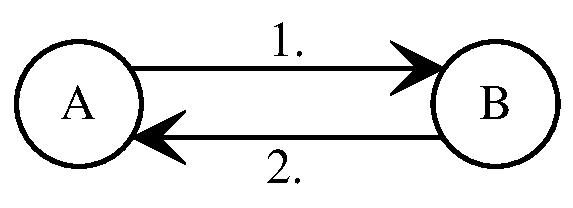
\includegraphics[width=0.5\textwidth]{pic/key_distribution-diffie-hellman}
    \caption{Общая схема взаимодействия участников в протоколе Диффи~---~Хеллмана\label{fig:key_distribution-diffie-hellman}}
\end{figure}

\begin{protocol}
    \item[(1)] Алиса выбирает случайное $2 \leq a \leq p - 1$
    \item[{}] $Alice \to \left\{ A = g ^ a \bmod p \right\} \to Bob$
    \item[(2)] Боб выбирает случайное $2 \leq b \leq p-1$
    \item[{}] Боб вычисляет сеансовый ключ $K = A ^ b \bmod p$
    \item[{}] $Bob \to \left\{ B = g ^ b \bmod p \right\} \to Alice$
    \item[(3)] Алиса вычисляет $K = B ^ a \bmod p$
\end{protocol}

Таким способом создан общий секретный сеансовый ключ $K$. За счёт случайного выбора значений $a$ и $b$ в новом сеансе будет получен новой сеансовый ключ.

Протокол обеспечивает только генерацию новых сеансовых ключей (цель G10). В отсутствие третей доверенной стороны он не обеспечивает ни аутентификацию сторон (цель G1), из-за отсутствия проходов с подтверждением владения ключом отсутствует аутентификация ключа (цель G8). Зато, так как протокол не использует длительные <<мастер>>-ключи, можно говорить о том, что он обладает свойством совершенной прямой секретности (цель G9).

Протокол можно использовать только с такими каналами связи, в которые не может вмешаться активный криптоаналитик. В противном случае протокол становится уязвим к простой <<атаке посередине>>.

\begin{figure}
    \centering
    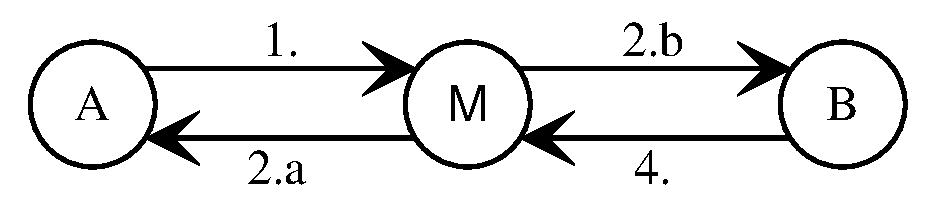
\includegraphics[width=0.67\textwidth]{pic/key_distribution-diffie-hellman-mitm}
    \caption{Схема взаимодействия участников в протоколе Диффи~---~Хеллмана в модели с активным криптоаналитиком\label{fig:key_distribution-diffie-hellman-mitm}}
\end{figure}

\begin{protocol}
    \item[(1)] Алиса выбирает случайное $2 \leq a \leq p - 1$
    \item[{}] $Alice \to \left\{ A = g ^ a \bmod p \right\} \to Mellory~(Bob)$
    \item[(2)] Меллори выбирает случайное $2 \leq m \leq p-1$
    \item[{}] Меллори вычисляет сеансовый ключ для канала с Алисой
        \[K_{AM} = A ^ m \bmod p = g ^ {am} \bmod p\]
    \item[{}] $Mellory~(Alice) \to \left\{ M = g ^ m \bmod p \right\} \to Bob$
    \item[{}] $Mellory~(Bob) \to \left\{ M = g ^ m \bmod p \right\} \to Alice$
    \item[(3)] Алиса вычисляет сеансовый ключ для канала с Меллори (думая, что Меллори это Боб)
        \[K_{AM} = M ^ a \bmod p = g ^ { am } \bmod p\]
    \item[(4)] Боб выбирает случайное $2 \leq b \leq p-1$
    \item[{}] Боб вычисляет сеансовый ключ для канала с Меллори (думая, что Меллори это Алиса)
        \[K_{BM} = M ^ b \bmod p = g ^ { bm } \bmod p\]
    \item[{}] $Bob \to \left\{ B = g ^ b \bmod p \right\} \to Mellory~(Alice)$
    \item[(5)] Меллори вычисляет сеансовый ключ для канала с Бобом
        \[K_{BM} = B ^ m \bmod p = g ^ { bm } \bmod p\]
\end{protocol}

В результате Алиса и Боб получили новые сеансовые ключи, но <<защищённый>> канал связи установили не с друг с другом, а со злоумышленником, который теперь имеет возможность ретранслировать или изменять все передаваемые сообщения между Алисой и Бобом.

Протокол Диффи~---~Хеллмана отличается от большей части протоколов распространения ключей из-за того, что не использует другие криптографические примитивы (функции шифрования, электронно-цифровой подписи или хеширования), но сам по себе является в некотором смысле криптографическим примитивом для построения более сложных протоколов. Он обеспечивает генерацию случайного числа в распределённой системе без доверенного центра. Причём ни одна из сторон не может заставить другую сторону использовать старый сессионный ключ, в отличие от, например, протокола Yahalom\index{протокол!Yahalom} из раздела~\ref{section-protocols-yahalom}.

Протокол можно изменить таким образом, чтобы вместо мультипликативной группы простого умножения использовать аддитивную группу сложения точек эллиптической кривой (см. раздел~\ref{section-math-ec-groups}). В этом случае стороны по прежнему будут выбирать некоторые случайные целые числа, но не возводить генератор-число в степень, а умножать генератор-точку на загаданное число.

\begin{protocol}
    \item[(0)] Стороны договорились о группе точек эллиптической кривой $\group{E}$, её циклической подгруппе $\group{G}$ мощности $n = \| \group{G} \|$ и генераторе $G$ группы $\group{G}$ (или хотя бы достаточно большой подгруппы группы $\group{G}$).
    \item[(1)] Алиса выбирает случайное $2 \leq a \leq n - 1$
    \item[{}] $Alice \to \left\{ A = a \times G \right\} \to Bob$
    \item[(2)] Боб выбирает случайное $2 \leq b \leq n - 1$
    \item[{}] Боб вычисляет точку $K = b \times A$
    \item[{}] $Bob \to \left\{ B = g \times G \right\} \to Alice$
    \item[(3)] Алиса вычисляет точку $K = a \times B$
\end{protocol}

В качестве нового сессионного ключа стороны могут выбрать, например, первую координату найденной точки $K$.


%\section{Протоколы с аутентификацией}

\subsection{Односторонняя аутентификация}

\textbf{Протокол Эль-Гамаля}\index{протокол!Эль-Гамаля} относится к протоколам с аутентификацией одного из двух легальных пользователей.
\selectlanguage{russian}
\begin{enumerate}
    \item Для начала стороны выбирают общие параметры $p, g$, где $p$ -- большое простое число, где $g$ -- примитивный элемент поля $\Z_p^*$.
    \item Сторона $B$ создает свои секретный и открытый ключи:
            \[ \SK_B = b, ~ \PK_B = g^b \mod p, \]
        $b$ -- случайное секретное число, $2 \leq b \leq p-1$.

        Открытый ключ $\PK_B$ находится в общем открытом доступе для всех сторон, поэтому криптоаналитик $E$ не может подменить его -- подмена будет заметна.
    \item Сторона $A$ вырабатывает свой секрет $x$, сеансовый ключ
            \[ K_A = (\PK_B)^x = g^{bx} \mod p \]
        и отправляет $B$:
            \[ A \rightarrow B: ~ g^x \mod p. \]
    \item Сторона $B$, получив от $A$ число $g^x \mod p$, использует его и свой секрет $\SK_B = b$, чтобы создать свой ключ
            \[ K_B = (g^x)^{\SK_B} = g^{bx} \mod p, \]
        то есть сеансовые ключи обеих сторон совпадают:
            \[ K_A = K_B = K. \]
\end{enumerate}

Достоинством этого протокола является следующее его свойство: если ключи $K_A$ и $K_B$ совпали и стороны могут обмениваться информацией, то сторона $A$ аутентифицирует сторону $B$, так как для шифрования она использовала открытый ключ $B$, который не может быть незаметно подменен, и только сторона $B$ может расшифровывать сообщения.

Что касается криптоаналитика в качестве <<человека-посередине>>, то он может отправлять ложные сообщения, но не может узнать ключ $K$ и читать сообщения.

Есть протоколы, в которых стороны, осуществляющие обмен информацией, являются равноправными. Они называются протоколами взаимной аутентификации.


\subsection{Взаимная аутентификация шифрованием}
\selectlanguage{russian}

К протоколам взаимной аутентификации принадлежит семейство протоколов, разработанных Т. Мацумото (T. Matsumoto), И. Такашима (Y. Takashima) и Х. Имаи (H. Imai) и названных по первым буквам фамилий авторов -- \textbf{протокол MTI}\index{протокол!MTI}.

Здесь к открытым данным относятся
    \[ p, ~~ g, ~~ \PK_A = g^a \mod p, ~~ \PK_B = g^b \mod p. \]
Каждый пользователь $A$ и $B$ обладает парой долговременных ключей для \emph{схемы шифрования с открытым ключом}: закрытый ключ расшифрования $\SK$ и открытый ключ шифрования  $\PK$.
\[ \begin{array}{ll}
    A: & ~ \SK_A = a, ~~ \PK_A = g^a \mod p, \\
    B: & ~ \SK_B = b, ~~ \PK_B = g^b \mod p. \\
\end{array} \]

\textbf{Протокол MTI}:
\begin{enumerate}
    \item Сторона $A$ генерирует случайное число $x, ~ 2\leq x\leq p-1$, создает и отправляет $B$ сообщение:
        \[ A \rightarrow B: ~ g^x \mod p. \]
    \item Сторона $B$ генерирует случайное число $y, ~ 2\leq y\leq p-1$, создает и отправляет $A$ сообщение:
        \[ A \leftarrow B: ~ g^y \mod p. \]
    \item Сторона $A$, используя открытые данные и полученное сообщение, создает сеансовый ключ:
        \[ K_A = (g^b)^x \cdot (g^y)^a = g^{bx+ay} \mod p. \]
    \item Сторона $B$, используя открытые данные и полученное сообщение, создает сеансовый ключ:
        \[ K_B = (g^x)^b \cdot (g^a)^y = g^{bx+ay} \mod p. \]
        Сеансовые ключи обоих сторон совпадают:
        \[ K_{A} =K_{B} = K. \]
\end{enumerate}

В описанном протоколе происходит взаимная аутентификация сторон как и в протоколе Эль-Гамаля\index{криптосистема!Эль-Гамаля}: открытые ключи сторон незаметно подменить невозможно. Наблюдая сообщения протокола, вычислить $g^{bx+ay}$ можно, только если известны значения $a,x$ или $b,y$, что представляет собой задачу дискретного логарифма, трудную в вычислительном смысле в настоящее время.


\subsection{Протокол Station-to-Station}\label{section-protocols-sts}\index{протокол!Station-to-Station|(}
\selectlanguage{russian}

Протокол STS (\langen{Station-to-Station},~\cite{Diffie:Oorschot:Wiener:1992})\index{протокол!Station-to-Station} предназначен для систем мобильной связи. Он использует идеи протокола Диффи~---~Хеллмана\index{протокол!Диффи~---~Хеллмана} и криптосистемы RSA\index{криптосистема!RSA}. Особенностью протокола является использование механизма электронной подписи\index{электронная подпись} для взаимной аутентификации сторон\index{аутентификация!взаимная}.

Предварительно стороны договорились об общих параметрах системы $p$ и $g$, где $p$ -- большое простое число, а $g$ -- примитивный элемент поля $\Z_p^*$.

Каждая из сторон $A$ и $B$ обладает долговременной парой ключей: закрытым ключом для расшифрования и создания электронной подписи $K_{\text{private}}$ и открытым ключом для шифрования и проверки подписи $K_{\text{public}}$.

\[\begin{array}{ll}
    A: K_{A,\text{private}}, K_{A,\text{public}}: \forall M : & \text{Verify}_A ( M, S_A( M ) ) = true, \\
                                                & D_A ( E_A( M ) ) = M, \\
    B: K_{B,\text{private}}, K_{B,\text{public}}: \forall M : & \text{Verify}_B ( M, S_B( M ) ) = true, \\
                                                & D_B ( E_B( M ) ) = M. \\
\end{array}\]

Где $\text{Verify}_A(\dots)$ это функция проверки электронной подписи на открытом ключе $K_{A, \text{public}}$, а $D_A$ -- функция расшифрования с использованием закрытого ключа $K_{A, \text{private}}$.

Протокол состоит из четырёх проходов, три из которых включают передачу сообщений (рис.~\ref{fig:key_distribution-sts}, \cite{Cheremushkin:2009}).

\begin{figure}
    \centering
    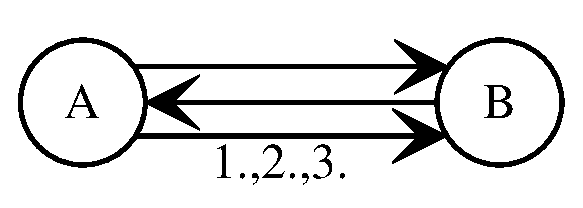
\includegraphics[width=0.5\textwidth]{pic/key_distribution-sts}
    \caption{Взаимодействие участников в протоколе STS\label{fig:key_distribution-sts}}
\end{figure}

\begin{protocol}
    \item[(1)] Алиса выбирает случайное число $R_A: 2 \leq R_A \leq p-1$.
    \item[{}] $Alice \to \left\{ A, m_A = g^{R_A} \bmod p \right\} \to Bob$

    \item[(2)] Боб выбирает случайное число $R_B: 2 \leq R_B \leq p-1$.
    \item[{}] Боб вычисляет сессионный ключ $K = m_A^{R_B} \bmod p$.
    \item[{}] $Bob \to \left\{ B, A, m_B = g^{R_B} \bmod p, E_K( S_B ( m_A, m_B )) \right\} \to Alice$

    \item[(3)] Алиса вычисляет сессионный ключ $K = m_B^{R_A} \bmod p$.
    \item[{}] Алиса проверяет подпись в сообщении $E_K( S_B ( m_A, m_B ))$.
    \item[{}] $Alice \to \left\{ A, B, E_K( S_A ( m_A, m_B ) ) \right\} \to Bob$

    \item[(4)] Боб проверяет подпись в сообщении $E_K( S_A ( m_A, m_B ))$.
\end{protocol}

Протокол обеспечивает гарантию формирования новых ключей (G10), но не совершенную прямую секретность (G9).

Как показала атака Лоу 1996 года (\cite{Lowe:1996}, рис.~\ref{fig:key_distribution-sts-attack}), протокол не может гарантировать аутентификацию субъектов (цель G1), ключей (G7) и подтверждение владения сессионным ключом (G8). Хотя злоумышленник не может получить доступ к новому сессионному ключу, если протокол использовать только для аутентификации субъектов, Алиса может принять злоумышленника за Боба.

\begin{figure}
    \centering
    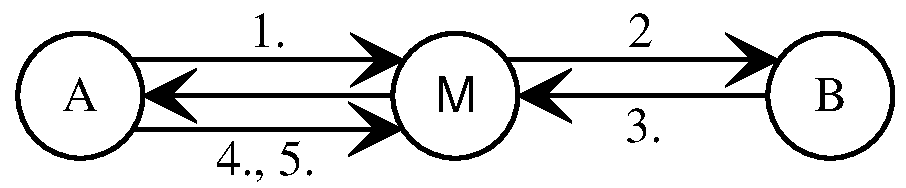
\includegraphics[width=0.67\textwidth]{pic/key_distribution-sts-attack}
    \caption{Схема взаимодействия участников в протоколе STS при атаке Лоу\label{fig:key_distribution-sts-attack}}
\end{figure}

\begin{protocol}
    \item[(1)] Алиса выбирает случайное число $R_A: 2 \leq R_A \leq p-1$.
    \item[{}] $Alice \to \left\{ A, m_A = g^{R_A} \bmod p \right\} \to Mellory~(Bob)$

    \item[(2)] $Mellory~(Alice) \to \left\{ M, m_A \right\} \to Bob$

    \item[(3)] Боб выбирает случайное число $R_B: 2 \leq R_B \leq p-1$ и вычисляет $m_B = g^{R_B} \bmod p$, а также сессионный ключ $K = m_A^{R_B} \bmod p$.
    \item[{}] $Bob \to \left\{ B, M, m_B, E_K( S_B ( m_A, m_B )) \right\} \to Mellory$

    \item[(4)] $Mellory~(Bob) \to \left\{ B, A, m_B, E_K( S_B ( m_A, m_B )) \right\} \to Alice$

    \item[(5)] Алиса вычисляет сессионный ключ $K = m_B^{R_A} \bmod p$.
    \item[{}] Алиса проверяет подпись в сообщении $E_K( S_B ( m_A, m_B ))$.
    \item[{}] $Alice \to \left\{ A, B, E_K( S_A ( m_A, m_B ) ) \right\} \to Mellory~(Bob)$
\end{protocol}

После успешного завершения протокола Алиса уверена, что общается с Бобом.

Как и все остальные <<криптосистемы-протоколы>>, протокол Station-to-Station основывается на некотором внешнем источнике информации об открытых ключах участников, не подвергая сомнению корректность и надёжность этого источника. Что, в общем случае, неверно. Если информацию о ключах участников нужно получать извне при каждом сеансе протокола (например, если участников много, и запомнить ключи всех возможности нет), то канал получения открытых ключей будет основной целью активного криптоаналитика для рассмотренных протоколов. Как от этого защититься с использованием примитивов асимметричной криптографии -- в разделе~\ref{section-protocols-asymmetric}.

\index{протокол!Station-to-Station|)}

\subsection{Схема Жиро}\label{section-girault-scheme}\index{схема!Жиро|(}
\selectlanguage{russian}

В схеме Жиро (\langfr{Marc Girault},~\cite{Girault:1990, Girault:1991}) надёжность строится на стойкости криптосистемы RSA (сложности факторизации больших чисел и вычисления дискретного корня).

Предварительно:
\begin{itemize}
    \item Доверенный центр (Трент, $T$):
    \begin{itemize}
        \item выбирает общий модуль $n = p \times q$, где $p$ и $q$ -- большие простые числа;
        \item выбирает пару из закрытого и открытого ключей $K_{T, \text{public}}: (e, n)$ и $K_{T, \text{private}}: (d, n)$;
        \item выбирает элемент $g$ поля $\mathbb{Z}_n^{\times}$ максимального порядка;
        \item публикует в общедоступном месте параметры схемы $n$, $e$ и $g$.
    \end{itemize}
    \item Каждый из легальных участников:
    \begin{itemize}
        \item выбирает себе закрытый ключ $s_i$ и идентификатор $I_i$;
        \item вычисляет и отправляет доверенному центру $v_i = g^{-s_i} \bmod n$;
        \item используя протокол аутентификации сторон (см. ниже) легальный участник доказывает доверенному центру, что владеет закрытым ключом, не раскрывая его значение;
        \item получает от доверенного центр свой открытый ключ:
            \[ P_i = (v_i - I_i)^d = (g^{-s_i} - I_i)^d \mod n; \]
    \end{itemize}
    В результате для каждого участника, например, Алисы, которая владеет $P_A, I_A, s_a$ будет выполняться утверждение:
        \[ P_A^e + I_A = g^{-s_A} \mod n. \]
\end{itemize}

Протокол аутентификации сторон в общем случае выглядит следующим образом (рис.~\ref{fig:key_distribution-girault-auth}).

\begin{figure}
    \centering
    \includegraphics[width=0.5\textwidth]{pic/key_distribution-girault-auth}
    \caption{Взаимодействия участников в протоколе идентификации Жиро\label{fig:key_distribution-girault-auth}}
\end{figure}

\begin{protocol}
    \item[(1)] Алиса выбирает случайное $R_A$.
    \item[{}] $Alice \to \left\{ I_A, P_A, t = g^{R_A} \right\} \to Bob$
    \item[(2)] Боб выбирает случайное $R_B$.
    \item[{}] $Bob \to \left\{ R_B \right\} \to Alice$
    \item[(3)] $Alice \to \left\{ y = R_A + s_A \times R_B \right\} \to Bob$
    \item[(4)] Боб вычисляет $v_A = P_A^e + I_A$;
    \item[{}] Боб проверяет, что $g^ y v_A^{R_B} = t$.
\end{protocol}

Протокол генерации сессионного ключа, либо просто \emph{схема Жиро}, как и другие схемы, состоит из проходов обмена открытой информацией и вычисления ключа (рис.~\ref{fig:key_distribution-girault-scheme}).

\begin{figure}
    \centering
    \includegraphics[width=0.5\textwidth]{pic/key_distribution-girault-scheme}
    \caption{Взаимодействие участников в схеме Жиро\label{fig:key_distribution-girault-scheme}}
\end{figure}

\begin{protocol}
    \item[(1)] $Alice \to \left\{ P_A, I_A \right\} \to Bob$
    \item[(2)] Боб вычисляет $K_{BA} = (P_A^e + I_A)^{s_B} \bmod n$.
    \item[{}] $Bob \to \left\{ P_B, I_B \right\} \to Alice$
    \item[(3)] Алиса вычисляет $K_{AB} = (P_B^e + I_B)^{s_A} \bmod n$.
\end{protocol}

В результате работы схемы стороны сгенерировали одинаковый общий сеансовый ключ.
\[ K_{AB} = (P_A^e + I_A)^{s_B} = (g^{-s_A})^{s_B} = g^{-s_As_B} \mod n; \]
\[ K_{BA} = (P_B^e + I_B)^{s_A} = (g^{-s_B})^{s_A} = g^{-s_As_B} \mod n; \]
            \[ K = K_{AB} = K_{BA} = g^{-s_As_B} \mod n. \]

Схема обеспечивает аутентификацию ключа (цель G7), так как только легальные пользователи смогут вычислить корректное значение общего сессионного ключа.

\index{схема!Жиро|)}

В этом разделе были рассмотрены протоколы, в которых ключи вырабатываются в процессе обмена информацией.
%Существует и другой подход, который будет рассмотрен в следующих разделах.